In the following section we will demonstrate the impact that the values of the cost function parameters and the similarity threshold can have in the incremental learning approach.
%
%It is the case that we obtain different learned models depending on the combination of such values.\\ \\
%
Two sets of experiments were conducted. The first set consists of evaluating the impact of giving priority to one of the four possible parameters that we take into consideration in our approach, which are: \textit{similarity threshold}, \textit{time cost}, \textit{functionality cost} and \textit{location cost}. While the second set consists of finding optimal combinations of parameters that lead to good incremental learning. 
%
\section{Experiment 1} 
For the first type of experiment we concentrate on learning one model, depicted in Figure \ref{experiment_model_example}, and also referred as \textit{original model}. The model is categorized as complex for this project because it involves a mixture of branched and sequential nodes.
%
We focus in this section on evaluating how the incremental learning approach performs when a particular parameter is prioritized. For this, we simply set the prioritized parameter to the value of 1 and the others to the minimum allowed value of 0.1. We do not experiment with values of 0 because that would completely ignore some parameters of our approach, and it would also contradict the nature of this project, as each parameter has a role in the process. 
%There exists four possible parameters that are used for incremental learning, therefore, we performed a set of four sub-experiments to analyze the behavior of the learning process with respect to the prioritized parameters. 
%
\begin{figure}[h]
	\centering
	\makebox[\textwidth][c]{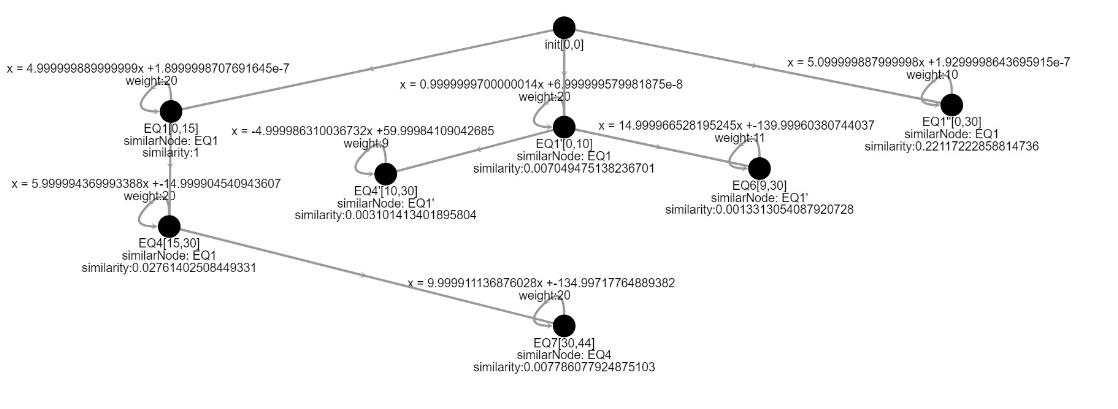
\includegraphics[width=1.0\textwidth]{./pictures/experiment.png}}%
	\caption{Experiment 1 Original Model}
	\label{experiment_model_example}
%	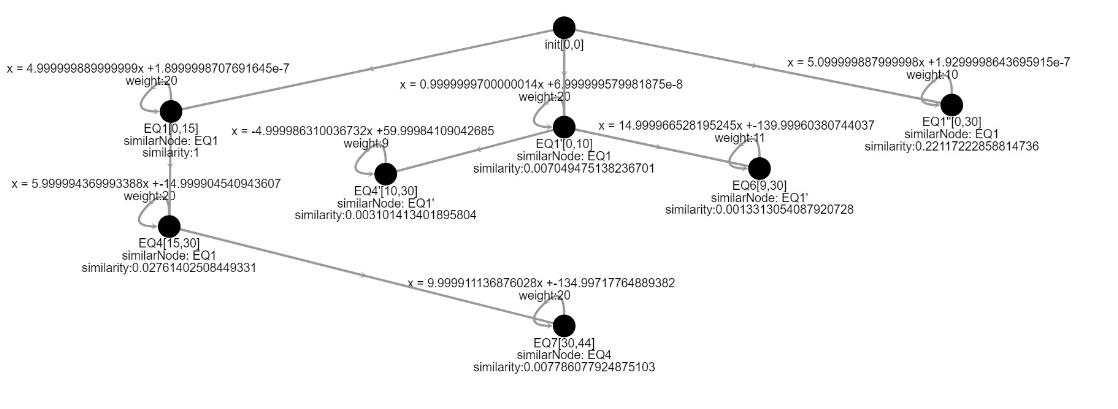
\includegraphics[scale=0.75]{./pictures/experiment.png}
\end{figure}

\subsection{Sub-Experiment 1 - Similarity Prioritized}
The \textit{Similarity threshold} is responsible for discriminating which learned nodes are close enough to be merged in the learning progress. In this experiment, its value is increased to 1, meaning that only completely identical locations will be considered in the evaluation of merging nodes via the cost function of our approach. 

\subsubsection{Results}
%We can see in Figure \ref{experiment_similarity_threshold} the structure of the final learned model. 
Despite the difference between the original model and the learned model from Figure \ref{experiment_similarity_threshold}, one can notice that the learned model actually contains the structure of the original one, but with additional nodes. 
\begin{figure}[h]
	\centering
	\includegraphics[scale=0.4]{./pictures/similarity_experiment/learnedModel.png}
	\caption{Sub-Experiment 1 - Similarity Prioritized - Learned Model}
	\label{experiment_similarity_threshold}
\end{figure}

\subsubsection{Evaluation}
The nature of this experiment can be explained by analyzing two particular learned models. The learned model from Figure \ref{experiment_similarity_threshold_1} represents the best performance of the learning approach, as all of the observations until that point were completely identical (e.g. Figure \ref{experiment_similarity_threshold_sim} in observation 10).
%
It is not until we see a slightly different observation, that the learned model begins to add redundant locations due to the strict criteria of the similarity threshold. One can see that the last two nodes (from left to right) of Figure \ref{experiment_similarity_threshold_2} are identical in terms of functionality, but were discovered in slightly different time ranges. Node \textit{EQ4"} was discovered in the time range of 10-30, while the other next to it was discovered in the range of 9-10. This minimal difference in time constraints is detected by the learner and therefore a new node is added, to not loose precision of the observed data.
%
Also being the reason that the replacement cost from Figure \ref{experiment_similarity_threshold_rep} always stays in 0, because we are only replacing identical locations, according to the similarity threshold of 1. Whenever there is a slight difference in the learned observations, a new node will be added. Therefore, one can see in Figure \ref{experiment_similarity_threshold_costs} that peaks, represent each node that was added to the learned model. It is also important to notice that from observation 43 until the end of the simulation (e.g. observation 100) the graph similarity stays constant because there are no new observations at any point. 
%
\newpage

\begin{figure}[h]
	\centering
	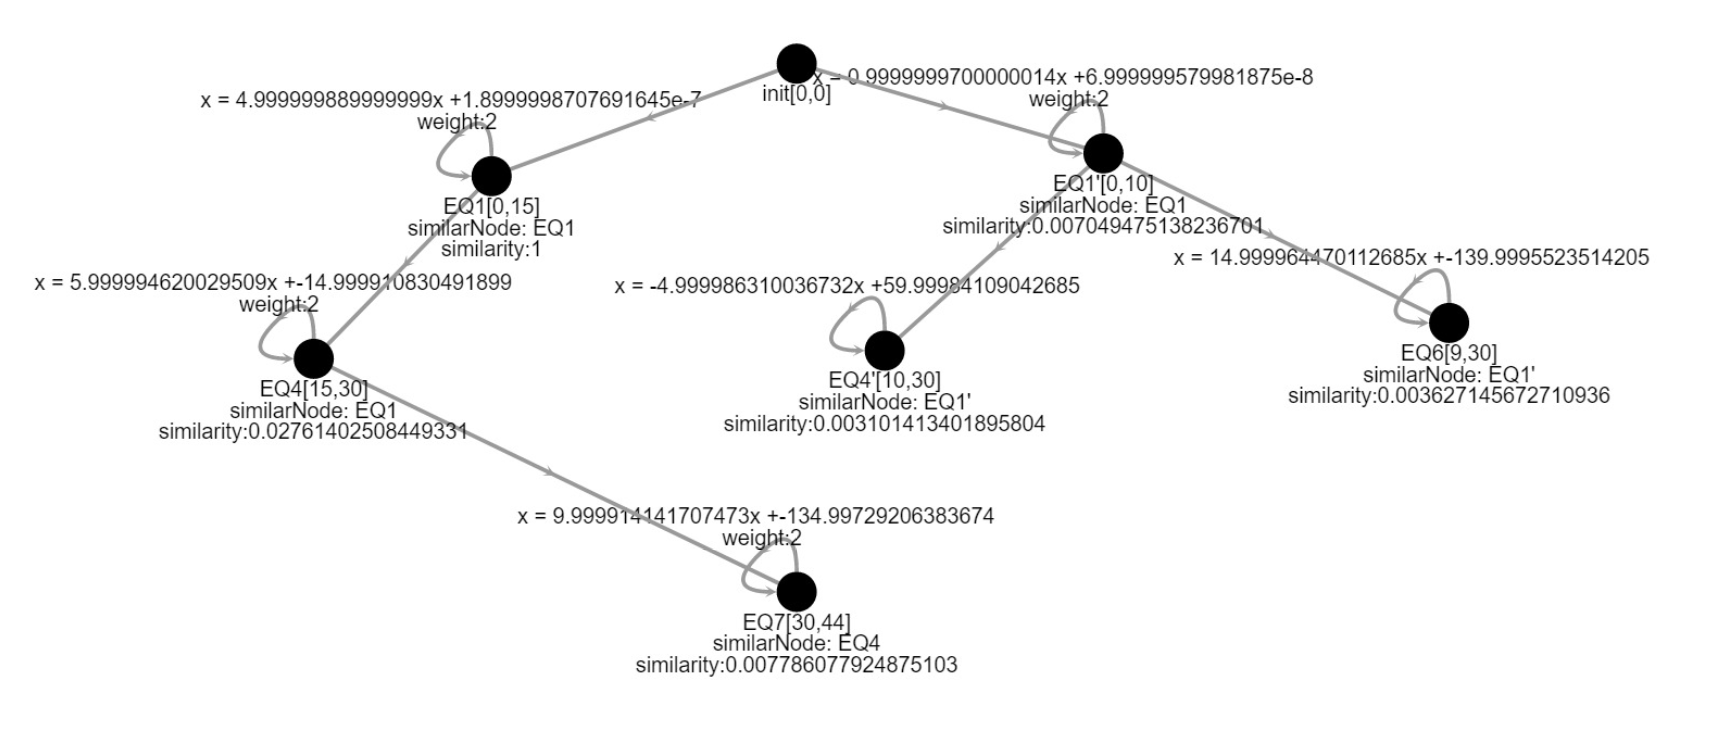
\includegraphics[scale=0.38]{./pictures/similarity_experiment/learnedModel_Obs10.png}
	\caption{Sub-Experiment 1 - Similarity Prioritized - Learned Model - Observation 10}
	\label{experiment_similarity_threshold_1}
\end{figure}

\begin{figure}[h]
	\centering
	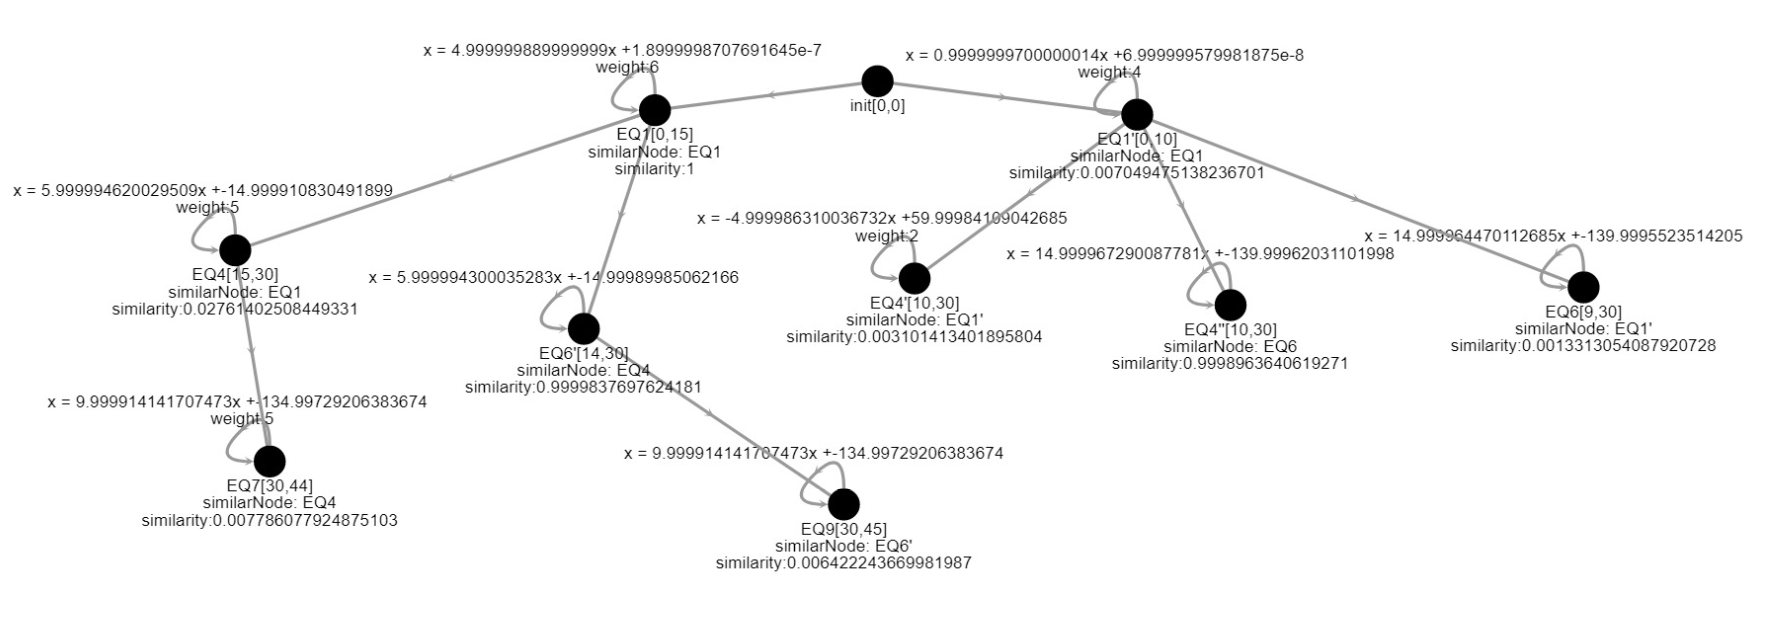
\includegraphics[scale=0.38]{./pictures/similarity_experiment/learnedModel_Obs26.png}
	\caption{Sub-Experiment 1 - Similarity Prioritized - Learned Model - Observation 26}
	\label{experiment_similarity_threshold_2}
\end{figure}

\newpage

\begin{figure}[h]
	\centering
	\includegraphics[scale=0.7]{./pictures/similarity_experiment/similarity.png}
	\caption{Sub-Experiment 1 - Similarity Prioritized - Graph Similarity}
	\label{experiment_similarity_threshold_sim}
\end{figure}

\newpage

\begin{figure}[h]
	\centering
	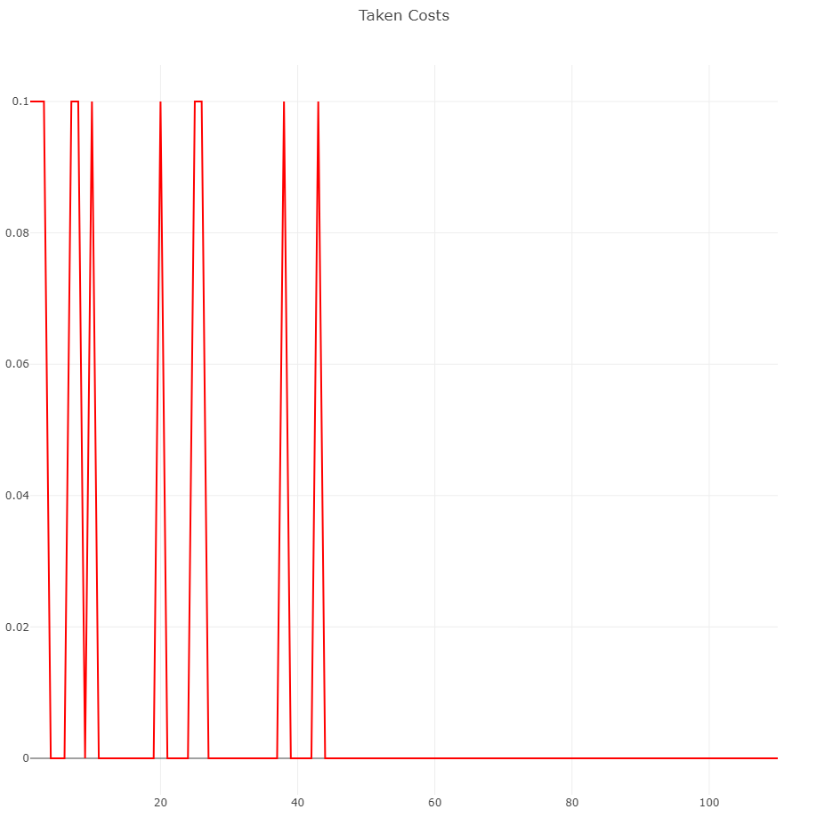
\includegraphics[scale=0.7]{./pictures/similarity_experiment/costs.png}
	\caption{Sub-Experiment 1 - Similarity Prioritized - Taken Costs}
	\label{experiment_similarity_threshold_costs}
\end{figure}

\begin{figure}[h]
	\centering
	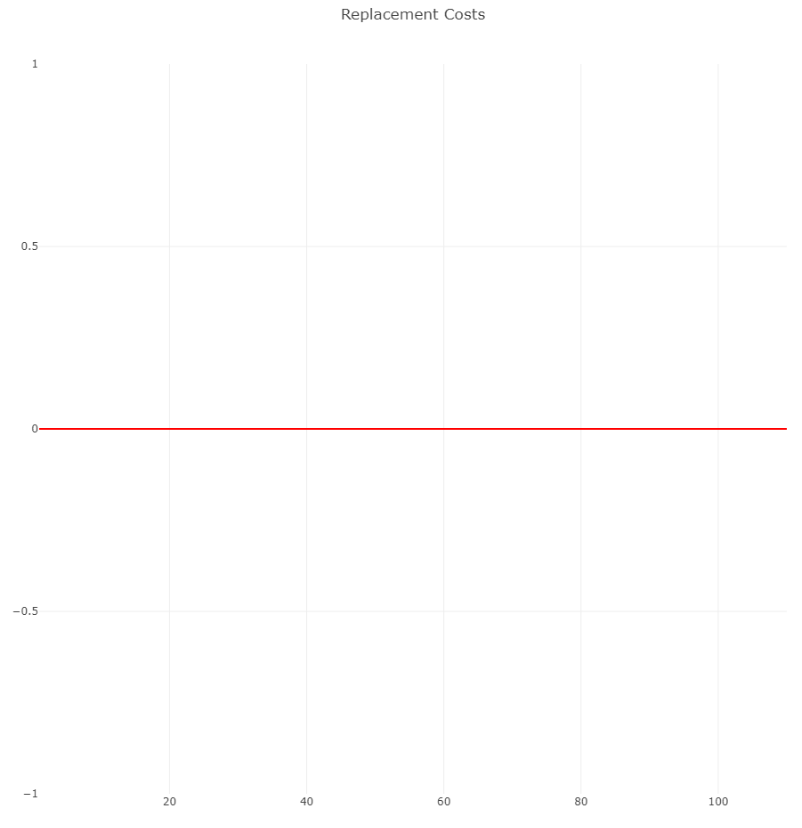
\includegraphics[scale=0.7]{./pictures/similarity_experiment/replacement.png}
	\caption{Sub-Experiment 1 - Similarity Prioritized - Replacement Costs}
	\label{experiment_similarity_threshold_rep}
\end{figure}

\newpage

\subsection{Sub-Experiment 2 - Time and Functionality Prioritized}
For this experiment the \textit{Time Cost} and \textit{Functionality Cost} will be set to 1 simultaneously. This is because the cost function explained in \Cref{chap:incremental_Learning}, calculates the error propagation of nodes based on the difference of time constraints and functionality among other nodes and incoming observations. Therefore, it is not meaningful to ignore one of the two criteria while evaluating observations. 

\subsubsection{Results}
In Figure \ref{time_func_experiment} we can see the final learned model. It is very interesting and also meaningful to notice that the structure resembles the one from the previous experiment in Figure \ref{experiment_similarity_threshold}. This is to be expected with the selected parameters, as the nodes must be almost identical when merging. Meaning that minimal differences in terms of functionality or time constraints will have a high cost, and will therefore lead to the addition of new nodes.

\begin{figure}[h]
	\centering
	\makebox[\textwidth][c]{\includegraphics[width=1.0\textwidth]{./pictures/time_functionality_experiment/learnedModel.png}}%
	\caption{Sub-Experiment 2 - Time and Functionality Prioritized - Learned Model}
	\label{time_func_experiment}
%	\includegraphics[scale=0.4]{./pictures/time_functionality_experiment/learnedModel.png}
\end{figure}

\subsubsection{Evaluation}
Despite the fact that we obtained the same learned model as in the previous experiment, the observations that caused the evolution of the model were not the same. Let us take a look at the peaks of the replacement costs from Figure \ref{time_func_experiment_rep}. Each peak represents an added location, as it is always the case that the cost of replacing a location surpasses the cost of adding one, due to the difference of time constraints and functionalities of nodes.
%
We can see in Figure \ref{time_func_experiment_sim_1} that the so far learned model contains an extra location on the bottom-right corner (e.g. node labeled as EQ6), causing the similarity to stay in 0.85 (as seen in Figure \ref{time_func_experiment_sim}), as the extra node could not be matched in the original model. In this particular case, the functionality cost did not play a role because node \textit{EQ4"} and \textit{EQ6} were identical in terms of functionality and only differed in time constraints by 1 time unit (same case as in the previous sub-experiment), causing the learner to add a new node to retain precision of the observations. \\ \\
%
Let us now pay attention to the highest peak from the graph shown in Figure \ref{time_func_experiment_rep}, as it represents the most expensive change that happened in the simulation. The reason of this peak is strongly related to the low value of the \textit{similarity threshold} (e.g. 0.1). 
%
In observation 38, a merge between node \textit{EQ1} and node \textit{EQ1"} (the opposite nodes of the first \textit{depth-level} of the graph) from the model shown in Figure \ref{time_func_experiment_sim_2} was attempted. 
%
This happened because the similarity of both nodes is 0.22 (number obtained by Algorithm \ref{measureDistances}), thus similar enough to be merged according the the similarity threshold value of 0.1.
%
Nevertheless, the merge was unsuccessful because there also existed difference in the time constraints. One node was observed in the range of 0-15 time units and the other one in the range of 0-30 time units. This accumulated a high cost of merging the two nodes because of their different time constraints. 
%
For this case, the functionality cost already showed a high cost that would have forced the learner to add a new node, but the difference in time constraints was also taken into account, causing the final cost to be very high. 
%
In the end, we could not perfectly learn the observed model mainly because of the strict parameters that were utilized while trying to merge similar nodes. The learned model is still adding redundant nodes of similar observations when they are not almost identical, as seen in each peak from Figure \ref{time_func_experiment_costs}. 
%
%
\begin{figure}[h]
	\centering
	\makebox[\textwidth][c]{\includegraphics[width=1.0\textwidth]{./pictures/time_functionality_experiment/learnedModel_Obs20.png}}%
	\caption{Sub-Experiment 2 - Time and Functionality Prioritized - Learned Model - Observation 20}
	\label{time_func_experiment_sim_1}
%	\includegraphics[scale=0.4]{./pictures/time_functionality_experiment/learnedModel_Obs20.png}
\end{figure}
%
\begin{figure}[h]
	\centering
	\makebox[\textwidth][c]{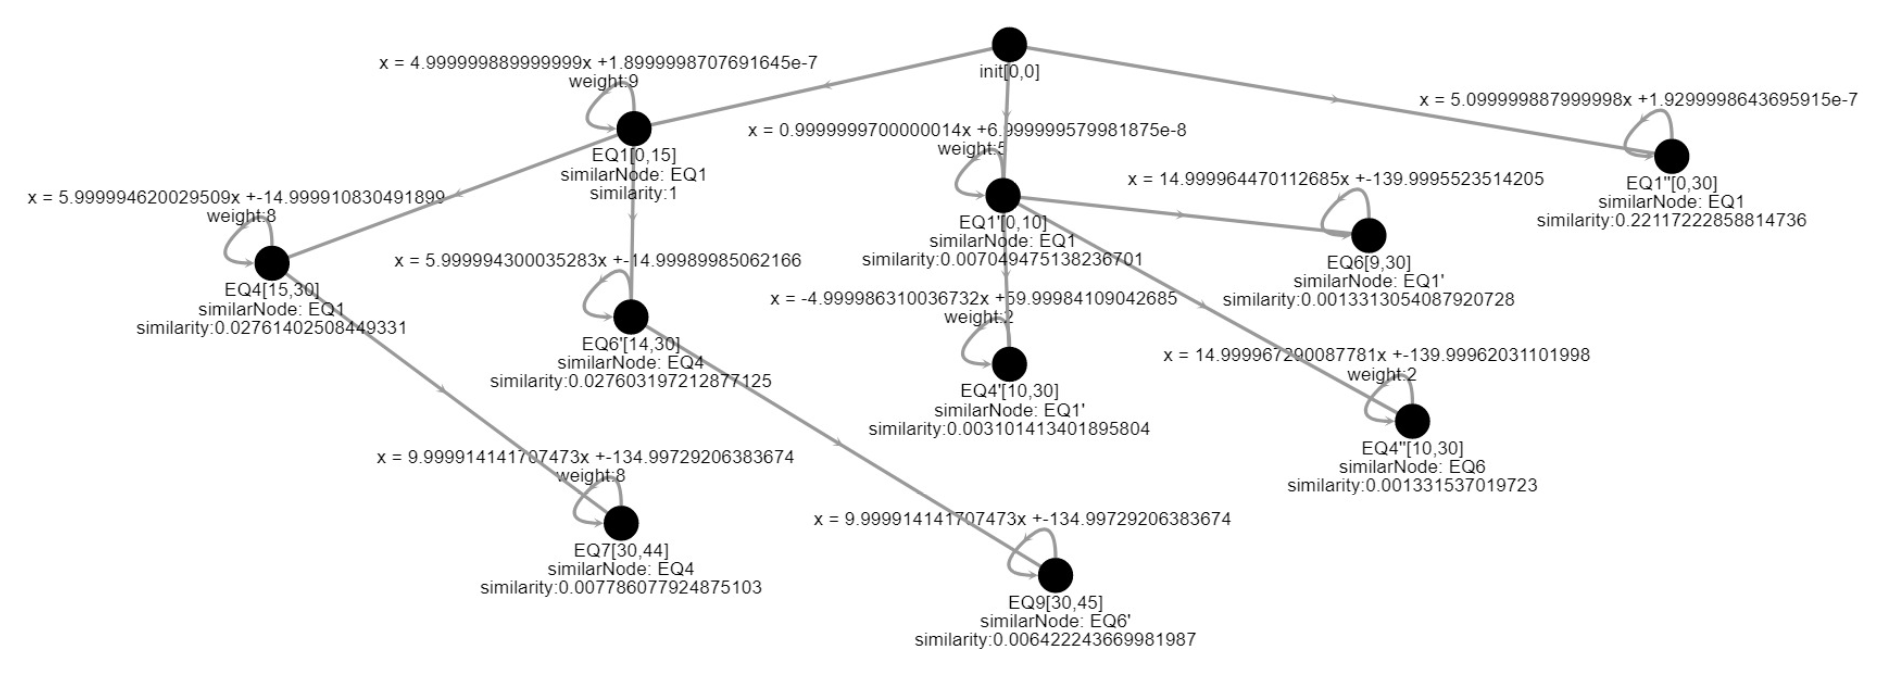
\includegraphics[width=1.0\textwidth]{./pictures/time_functionality_experiment/learnedModel_Obs38.png}}%
	\caption{Sub-Experiment 2 - Time and Functionality Prioritized - Learned Model - Observation 38}
	\label{time_func_experiment_sim_2}
%	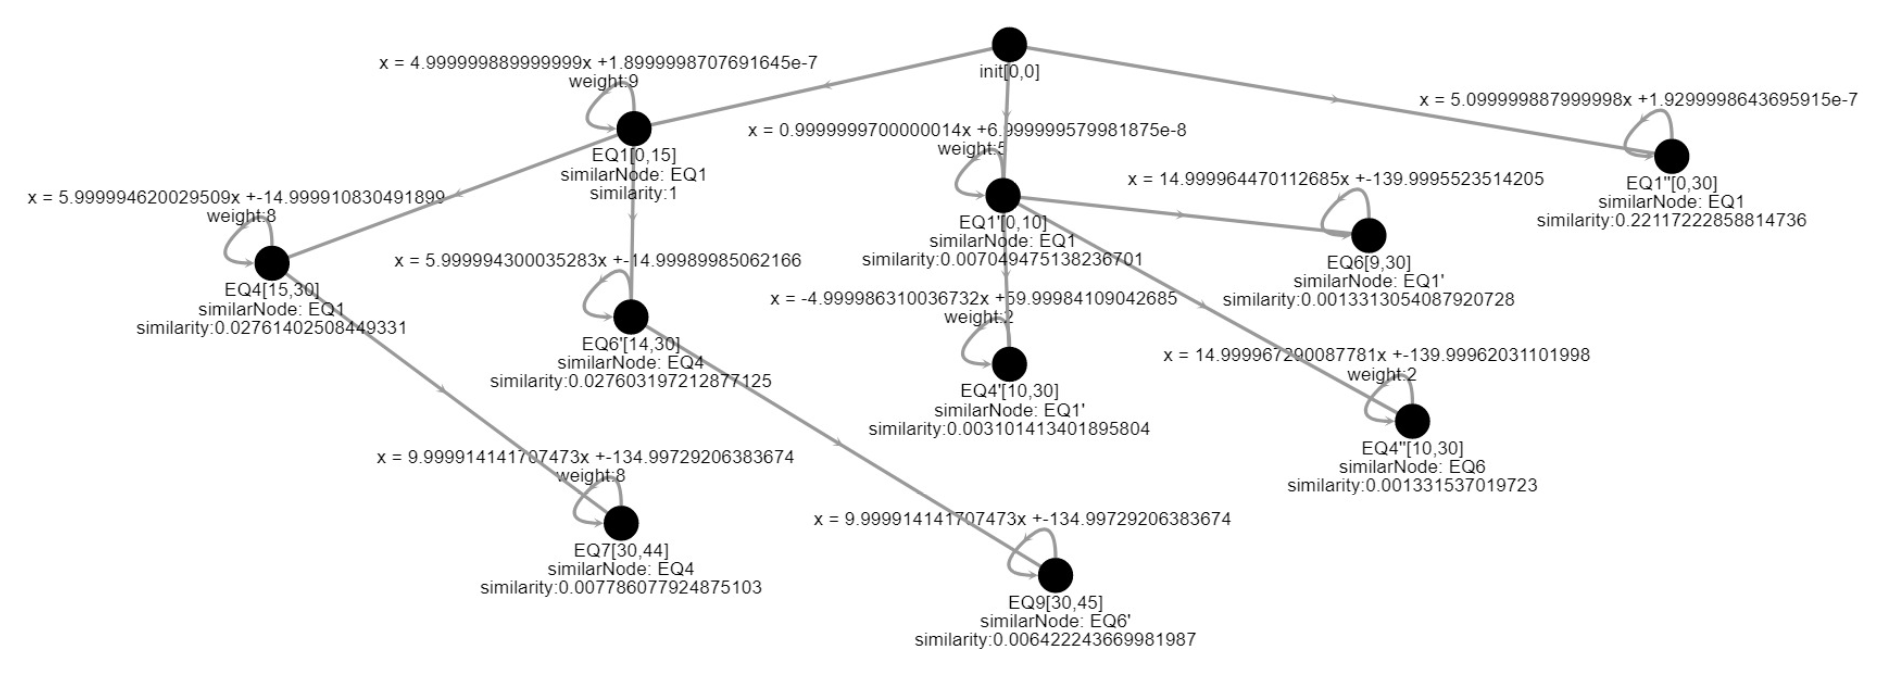
\includegraphics[scale=0.4]{./pictures/time_functionality_experiment/learnedModel_Obs38.png}
\end{figure}
%
\newpage

\begin{figure}[h]
	\centering
	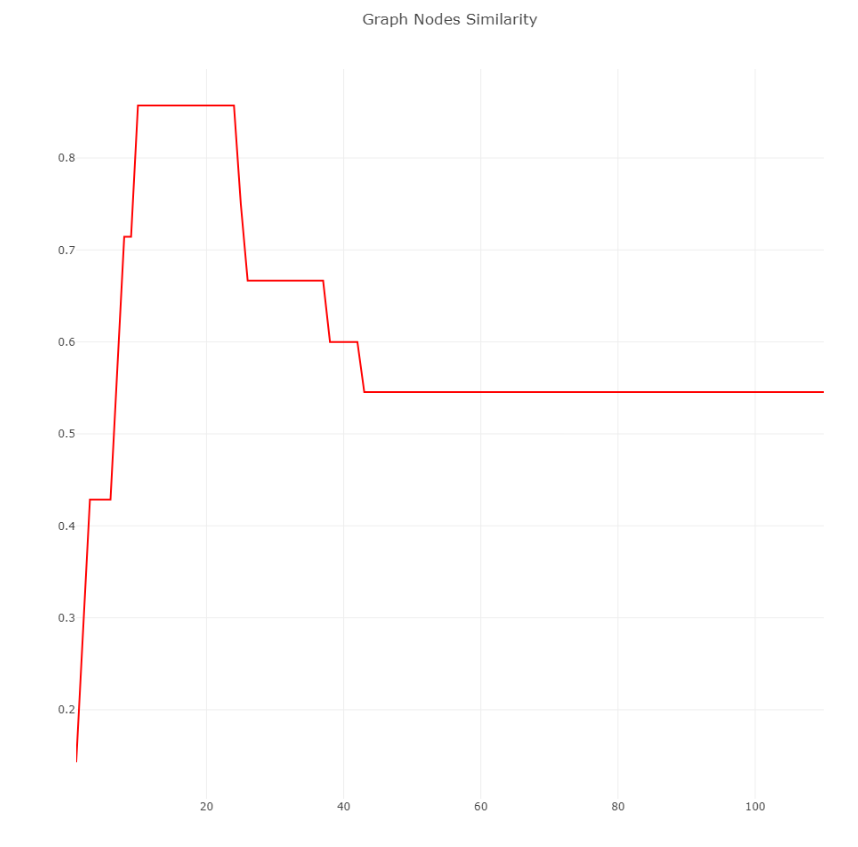
\includegraphics[scale=0.7]{./pictures/time_functionality_experiment/similarity.png}
	\caption{Sub-Experiment 2 - Time and Functionality Prioritized - Graph Similarity}
	\label{time_func_experiment_sim}
\end{figure}
%
\newpage
%
\begin{figure}[h]
	\centering
	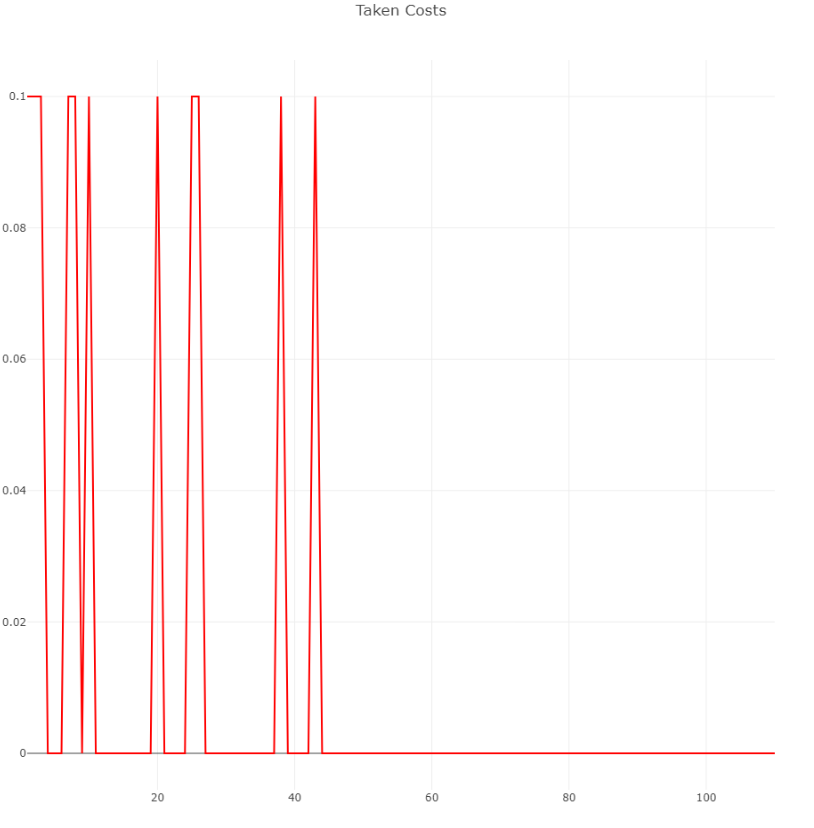
\includegraphics[scale=0.5]{./pictures/time_functionality_experiment/costs.png}
	\caption{Sub-Experiment 2 - Time and Functionality Prioritized - Taken Costs}
	\label{time_func_experiment_costs}
\end{figure}
%
\newpage
%
\begin{figure}[h]
	\centering
	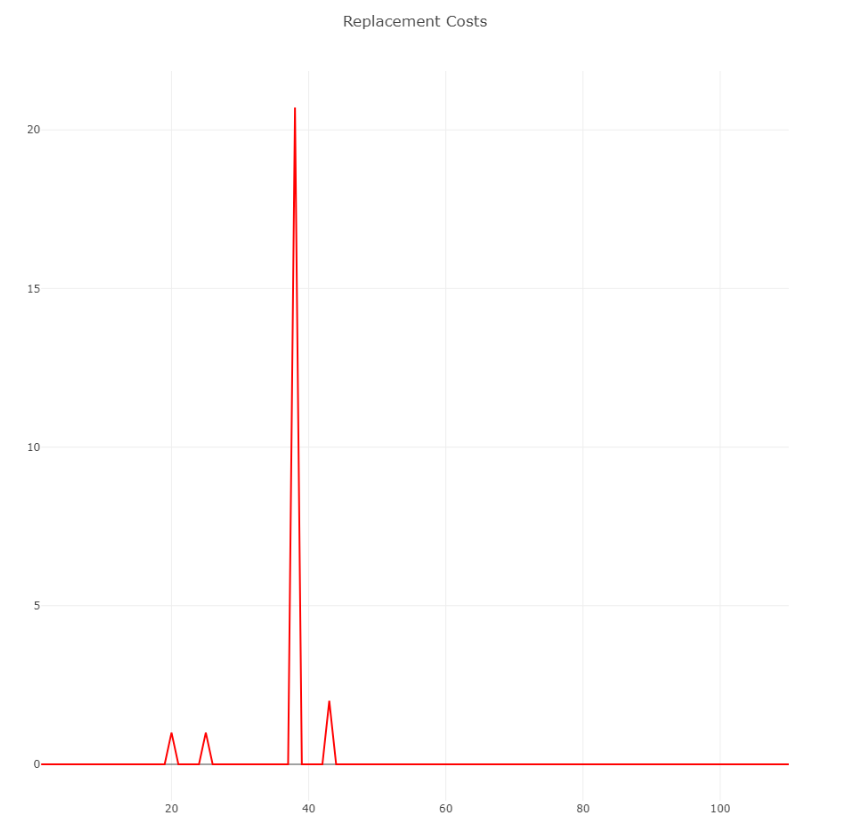
\includegraphics[scale=0.5]{./pictures/time_functionality_experiment/replacement.png}
	\caption{Sub-Experiment 2 - Time and Functionality Prioritized - Replacement Costs}
	\label{time_func_experiment_rep}
\end{figure}

\subsection{Sub-Experiment 3 - Node Addition Prioritized}
In this final experiment we set a high cost for adding locations (e.g. 1.0), while the other parameters are set to a low value (e.g. 0.1). Meaning that the learned model will be able to merge slight changes or noise from observations without needing to add an extra node every time that a different observation is learned. 

\subsubsection{Results}
As seen in Figure \ref{addition_experiment}, the learned model completely matches the original one. It was the case in this experiment because the learning process gave more priority (or cost) to the addition of new nodes. Which means that nodes that were added in the learned model were very distinguished among others in terms of time constraints and functionality, while similar nodes and observations were merged. 

\begin{figure}[h]
	\centering
	\makebox[\textwidth][c]{\includegraphics[width=1.0\textwidth]{./pictures/addition_experiment/learnedModel.png}}%
	\caption{Sub-Experiment 3 - Node Addition Prioritized - Learned Model}
	\label{addition_experiment}
%	\includegraphics[scale=0.4]{./pictures/addition_experiment/learnedModel.png}
\end{figure}

\subsubsection{Evaluation}
As we know that the original model was successfully learned, we will explain in detail why that was the reason by interpreting two particular observations that made the difference in the learning process. Looking at the first peak of Figure \ref{addition_experiment_rep}, the observation number 20 perfectly matched the functionality of node \textit{EQ6} (node located at the medium-right corner of Figure \ref{addition_experiment_sim_1}), with the only difference of 1 time unit from the observed time constraints. In the previous experiments, this difference of time would have caused the learning process to add an extra node to express the observation. 
%
But for this experiment it is not the case, as the cost of merging minimal time constraints and functionalities of nodes is very low. Therefore, despite the minimal difference in time constraints, the learned model ignores the unseen time unit to keep a minimal number of nodes, but it also sacrifices some precision of the information learned.
%
Although, if we take a look at the highest peak of the previous graph, one can easily see that the cost of replacing a node is higher than the one of adding a new one. The reason of this high cost is because a new observation was discovered in that point (e.g. the top-right node \textit{EQ1"} from Figure \ref{addition_experiment}). This last added node could not be merged with the closest node found (node \textit{EQ1} located at the top-left corner from the same figure) mainly due to their differences in terms of functionality and time constraints. The functionality differed by 0.2 (e.g. Euclidean distance calculated by Algorithm \ref{measureDistances}) and the number of unseen times were 15 (as in the sub-experiment 2). Given the flexibility of the learned to merge similar nodes, this difference was considered great enough to discard the merging procedure and to add the observation as a new node. At this point, it is important to remark that if the nodes were to be merged, we could have had fewer locations in our learned model and less precision in the data. But this change would have caused the similarity of our models to decrease significantly.
%
%in this case, it also did not succeed to do so because the difference in functionality and time constraints was high enough to express th observation as a new node. Otherwise the merge of the nodes would have propagated significant errors to the learned model. 
%
Consequently, one can see in Figure \ref{addition_experiment_costs} that the cost of adding a node (e.g. 1.0) was taken instead of the one of merging nodes (e.g. 2.0). And it is indeed from this point the no new significant behavior was learned from the observations, as the similarity between the original model and the learned model remained optimal and constant, as depicted in Figure \ref{addition_experiment_sim}
%
\newpage

\begin{figure}[h]
	\centering
	\includegraphics[scale=0.4]{./pictures/addition_experiment/learnedModel_Obs20.png}
	\caption{Sub-Experiment 3 - Node Addition Prioritized - Learned Model - Observation 20}
	\label{addition_experiment_sim_1}
\end{figure}

\newpage

%%
%\begin{figure}[h]
%	\centering
%	\caption{Sub-Experiment 1 - Similarity Prioritized - Learned Model - Observation 38}
%	\label{time_func_experiment_sim_2}
%	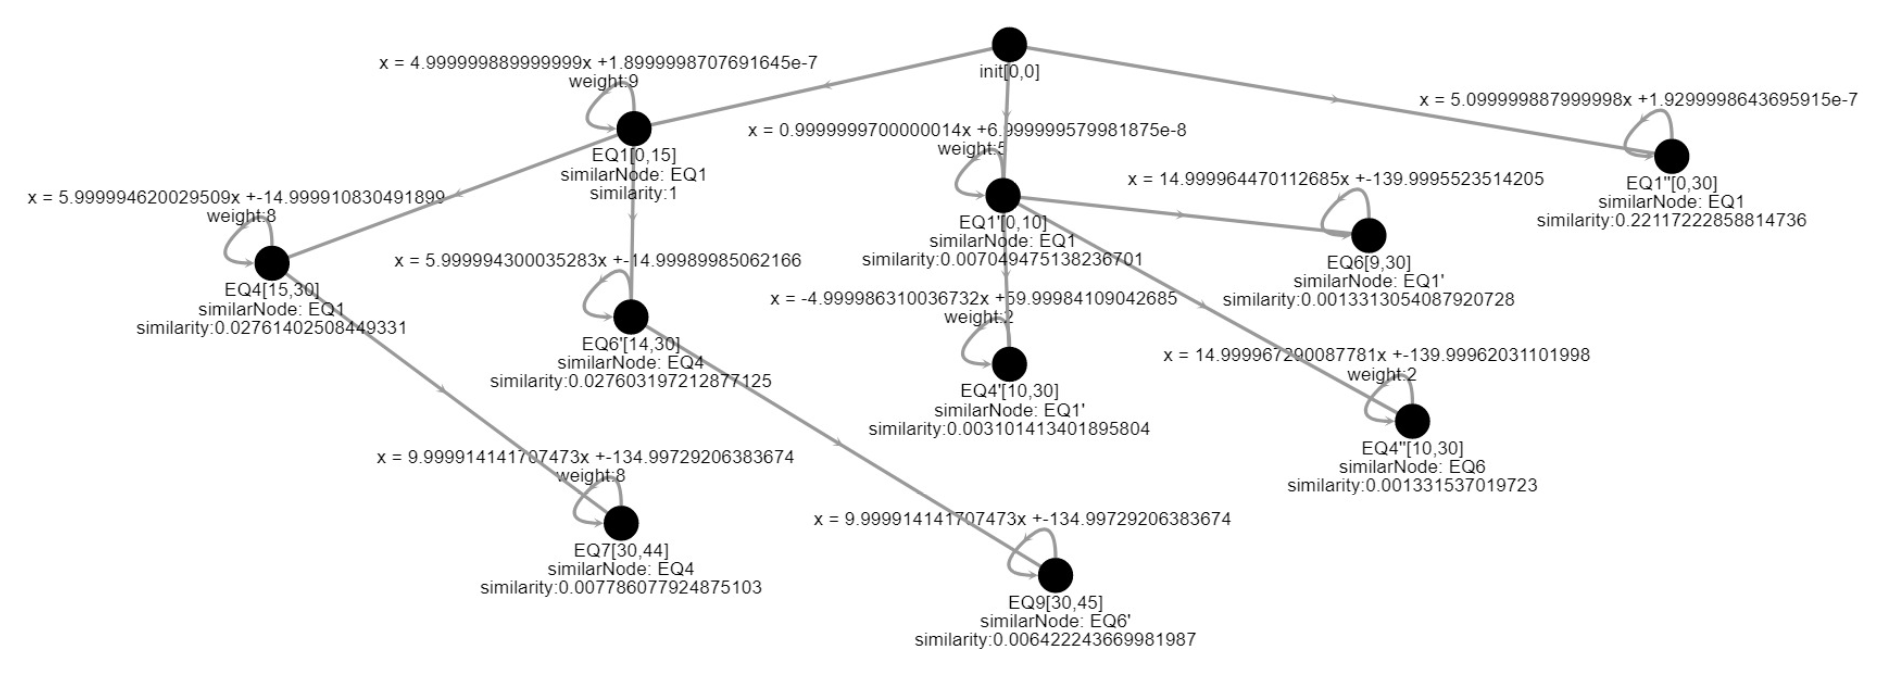
\includegraphics[scale=0.4]{./pictures/time_functionality_experiment/learnedModel_Obs38.png}
%\end{figure}
%%
\begin{figure}[h]
	\centering
	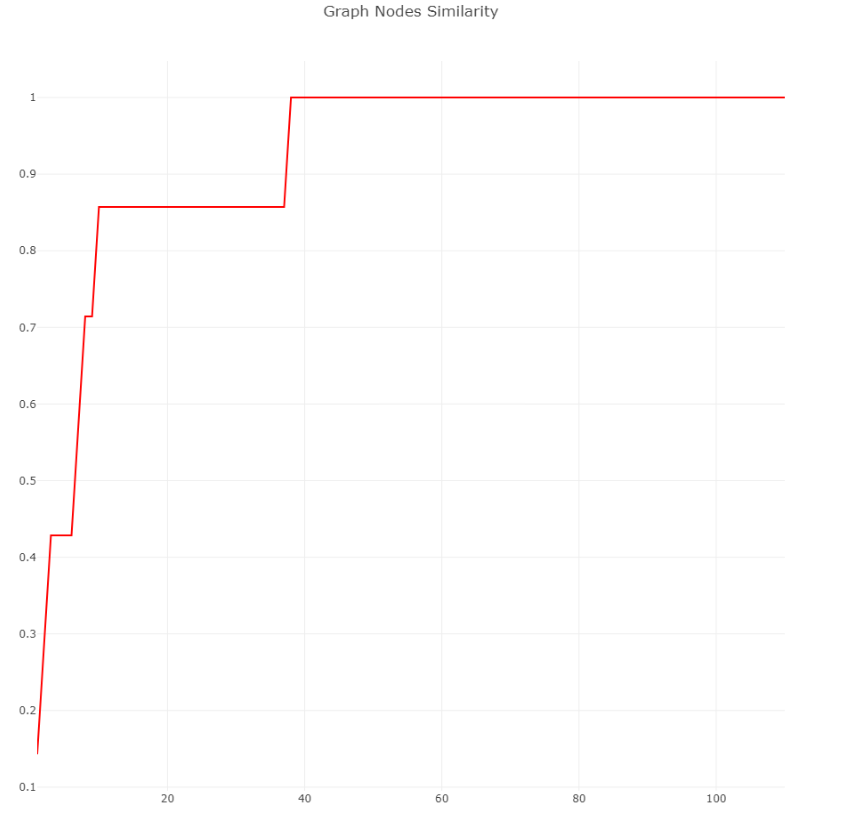
\includegraphics[scale=0.7]{./pictures/addition_experiment/similarity.png}
	\caption{Sub-Experiment 3 - Node Addition Prioritized - Graph Similarity}
	\label{addition_experiment_sim}
\end{figure}
%
\newpage

\begin{figure}[h]
	\centering
	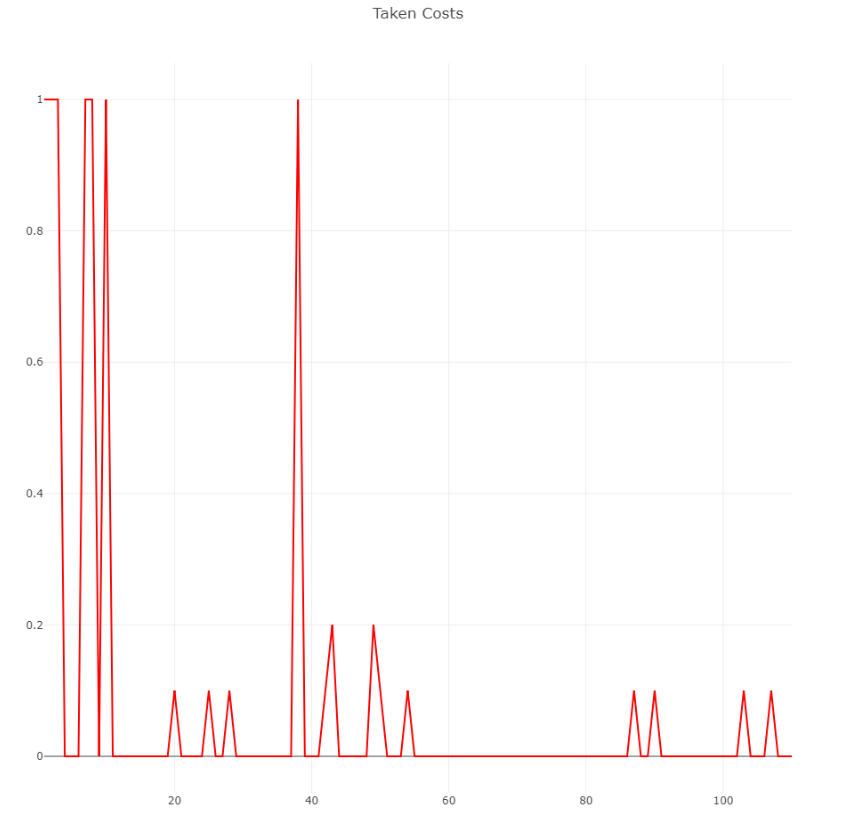
\includegraphics[scale=0.5]{./pictures/addition_experiment/costs.png}
	\caption{Sub-Experiment 3 - Node Addition Prioritized - Taken Costs}
	\label{addition_experiment_costs}
\end{figure}
%
\begin{figure}[h]
	\centering
	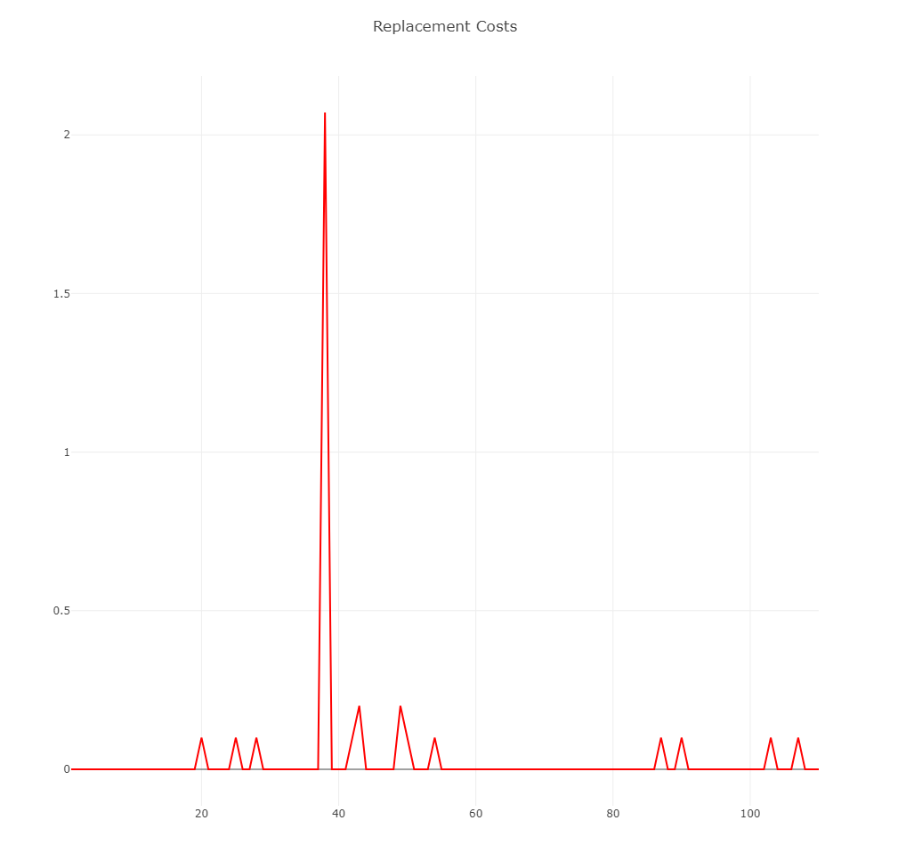
\includegraphics[scale=0.5]{./pictures/addition_experiment/replacement.png}
	\caption{Sub-Experiment 3 - Node Addition Prioritized - Replacement Costs}
	\label{addition_experiment_rep}
\end{figure}

\newpage

\section{Experiment 2}
After observing how the incremental learning process behaves differently given prioritized parameters, in this section we attempt to find the optimal combination of parameters in which an observed model can be learned. In the previous experiment, we restricted ourselves to one type of combination and to two possible values (e.g. 0.1 and 1) for the \textit{cost parameters} and \textit{similarity threshold}. In this experiment we restrict ourselves to three different values: 0.1, 0.5, and 1, but with the possibility of allowing different combinations of them while learning observations. Therefore, we divided this section into two sub-experiments. In the first sub-experiment we learn a model with combinations of branches and sequential nodes. Whereas in the second sub-experiment we learn two simple and relatively small models. The purpose of this division is to demonstrate how the learning process behaves with different types of models.

\subsection{Sub-Experiment 1}
We used the same model as in Experiment 1 (e.g. Given in Figure \ref{experiment_model_example}), and learned it once again by using 81 combinations of different parameters for the \textit{cost function} and the \textit{similarity threshold}.

\subsubsection{Results}
At the end, 63 combinations could match 54\% of the original model (learned model in Figure \ref{combination_experiment_1}), 6 out of 81 matched 70\% of original model (learned model in Figure \ref{combination_experiment_2}), and only 12 combinations could match it by 100\%. 
% 
\begin{figure}[h]
	\centering
	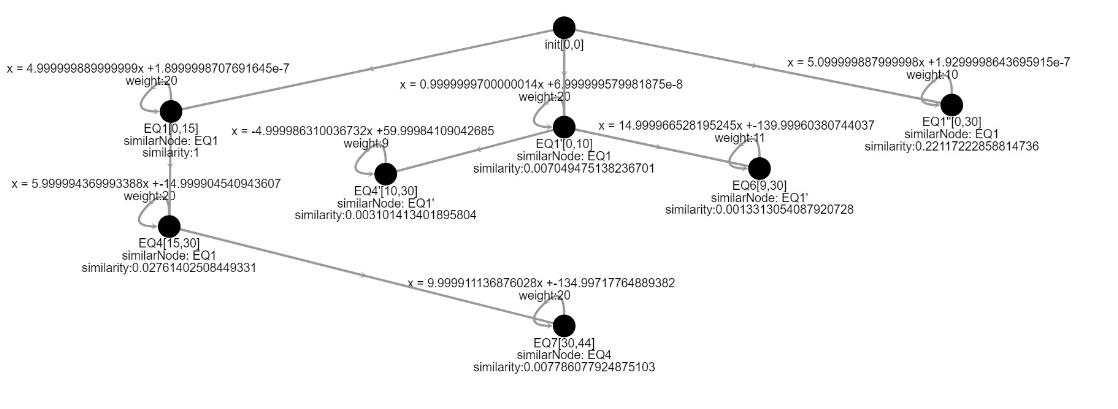
\includegraphics[scale=0.6]{./pictures/experiment.png}
	\caption{Sub-Experiment 1 - Original Model}
	\label{combination_experiment_model}
\end{figure}

\begin{figure}[h]
	\centering
	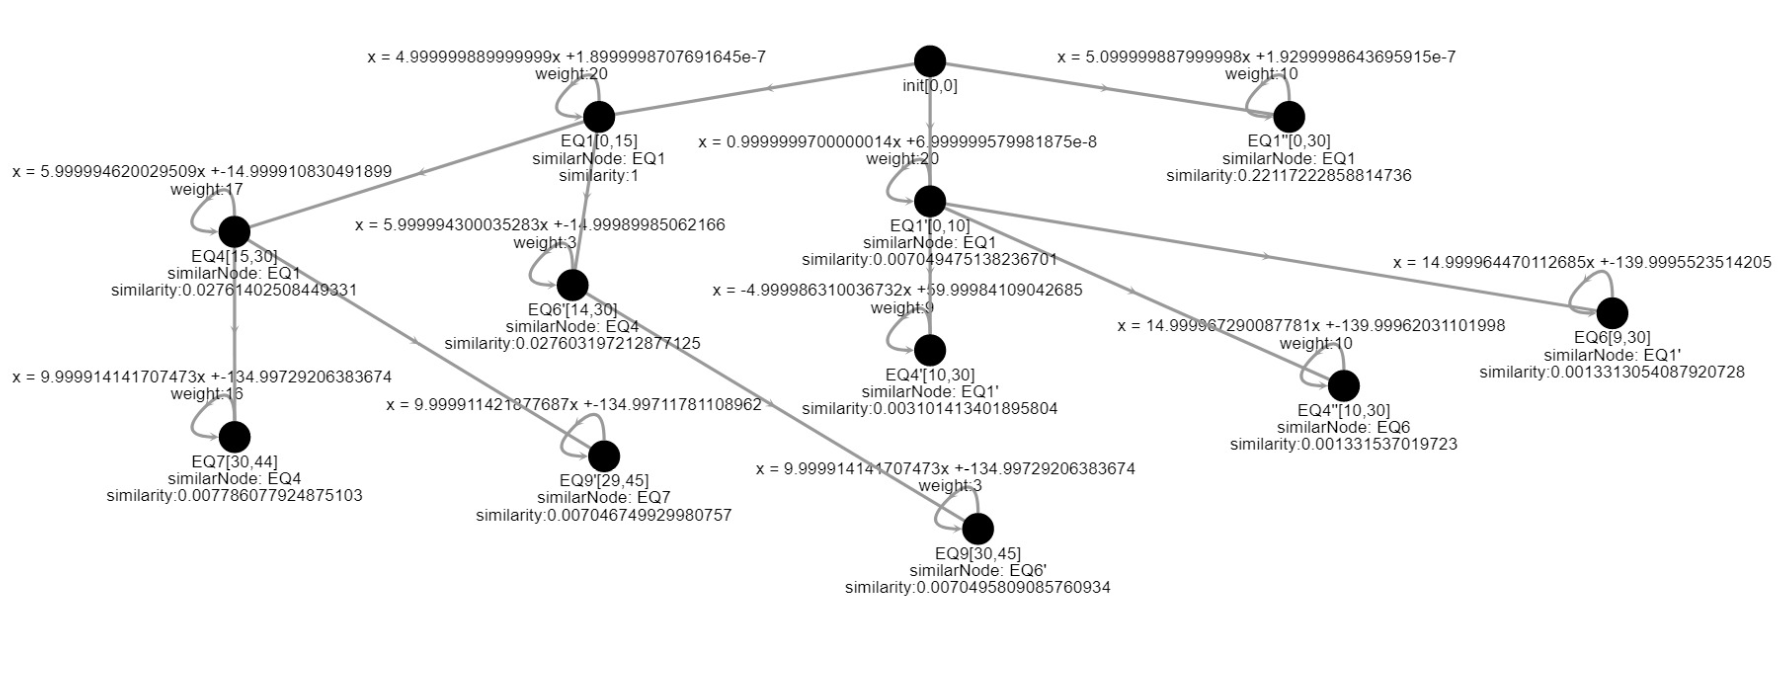
\includegraphics[scale=0.4]{./pictures/combination_experiment/learnedModel_worse.png}
	\caption{Sub-Experiment 1 - 54\% of original mode learned}
	\label{combination_experiment_1}
\end{figure}

\begin{figure}[h]
	\centering
	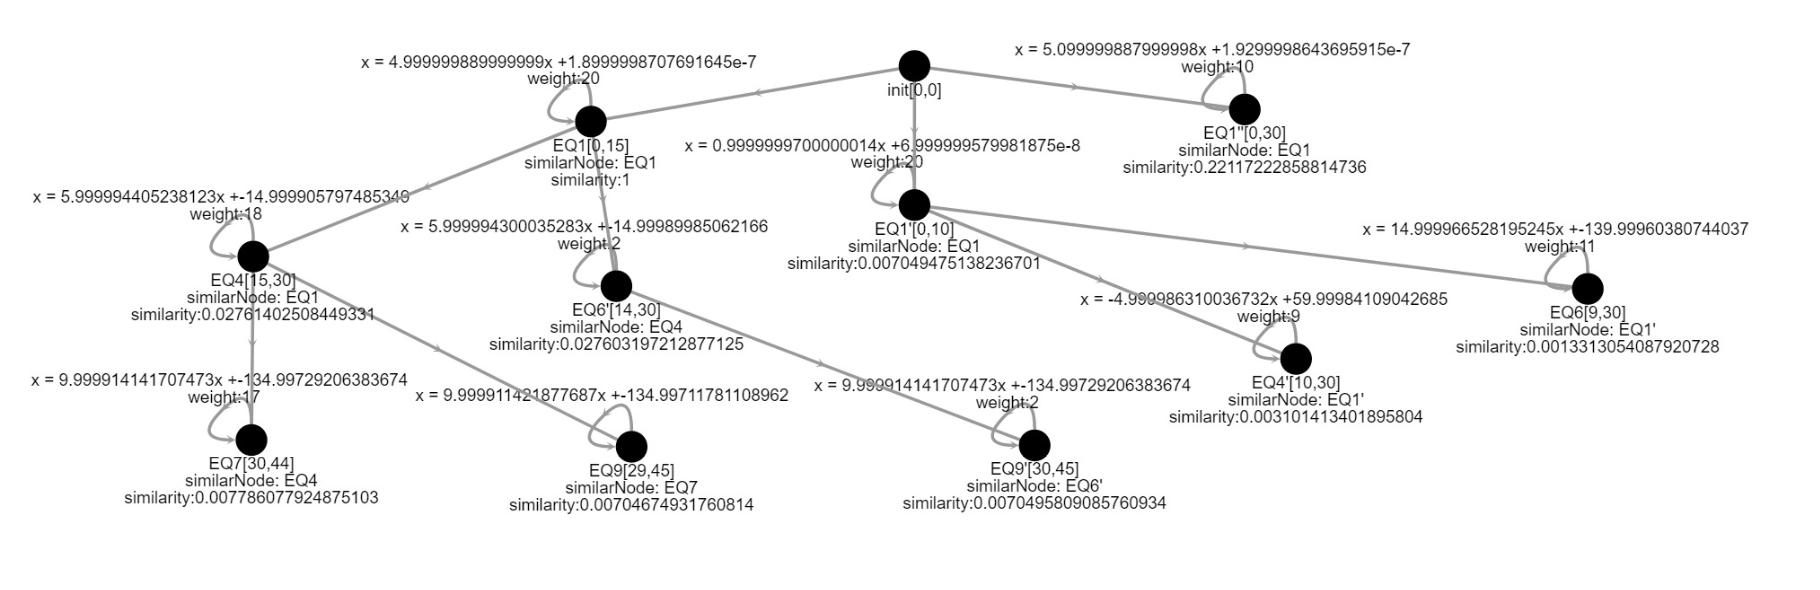
\includegraphics[scale=0.4]{./pictures/combination_experiment/learnedModel_better.png}
	\caption{Sub-Experiment 1 - 70\% of original mode learned}
	\label{combination_experiment_2}
\end{figure}

%\begin{figure}[h]
%	\centering
%	\caption{Experiment 2 - Graph Similarities}
%	\label{addition_experiment_costs}
%	\includegraphics[scale=0.5]{./pictures/combination_experiment/similarity.png}
%\end{figure}
%%
%\begin{figure}[h]
%	\centering
%	\caption{Experiment 2  - Replacement Costs}
%	\label{addition_experiment_rep}
%	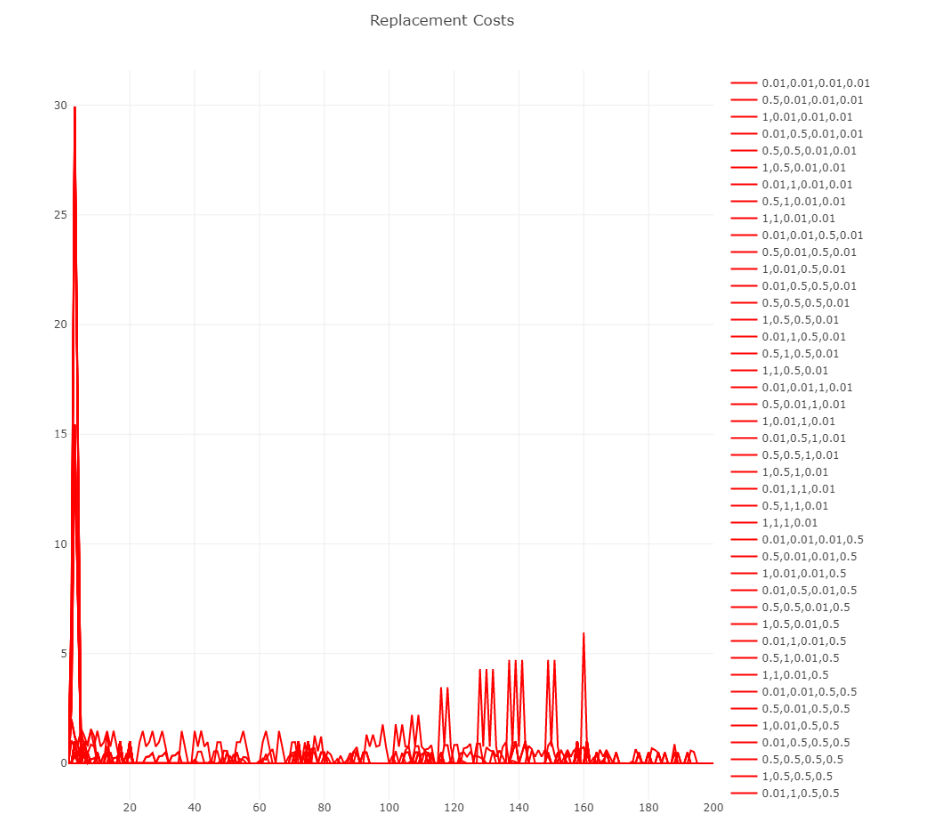
\includegraphics[scale=0.5]{./pictures/combination_experiment/replacement.png}
%\end{figure}
%\begin{figure}[h]
%	\centering
%	\caption{Experiment 2  - Taken Costs}
%	\label{addition_experiment_costs}
%	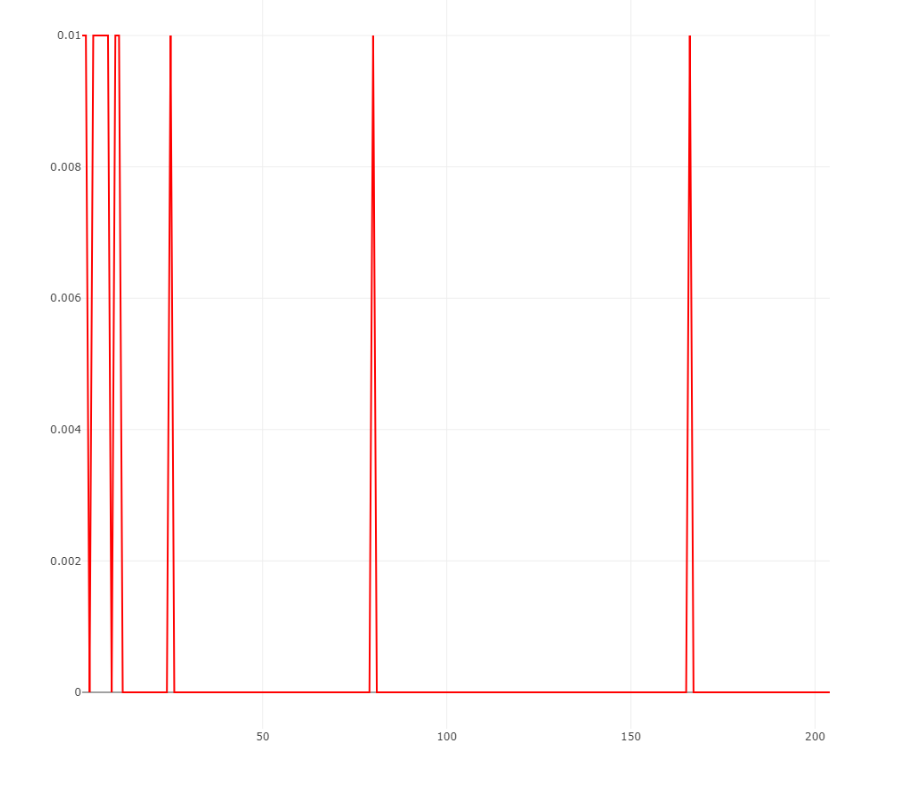
\includegraphics[scale=0.5]{./pictures/combination_experiment/costs.png}
%\end{figure}

\newpage
\subsubsection{Evaluation}
In the following tables we can see exactly which set of combination accomplished to learn the models mentioned previously. Each table will be analyzed separately and the conclusion of this experiment will be drawn until the end of this section.\\ \\
%
Let us first take a look when the original model could be learned completely in Table \ref{table:combination_1}. We can see that  the \textit{similarity threshold} never reached 1.0 and that the time constraints were given low priority at all times. In contrast to the \textit{location cost} which never reached the value of 0.1. It was for almost all of the cases that the model could be perfectly learned, by only giving priority to the functionalities of the observations and the overall number of nodes required to express observations. \\ \\
%
In Table \ref{table:combination_2} one can see the combinations when 70 \% of the model could be learned. It was the case that raising the priority of the \textit{time cost} had a negative effect on the learning process, despite the fact that the \textit{cost function} and \textit{location cost} remained relatively similar.  As seen in Figure \ref{combination_experiment_2}, this combination could not learned the model completely, only because two different time units of unique nodes were observed (nodes \textit{EQ7} and \textit{EQ9} from the same figure). \\ \\
%
At last, we will discuss Table \ref{table:combination_3}, were the worst combinations can be appreciated. In the majority of the cases, the model was wrongly learned whenever only identical observations were possible to merge (e.g. similarity threshold equal to 1). This is to be expected, as with a high \textit{similarity threshold}, the learned model does not tolerate any noisy or slightly modified observations. The same applies whenever the \textit{time cost} was set to a high value, as some of the observations had different time constraints and identical behaviors.  \\ \\
%
For this specific experiment, it was enough to ignore the minimal noise of the time constraints of the observations, and to separate the observations based on they're functionalities because they were relatively far between each other. 

\begin{table}[htbp]
	\centering
	\resizebox{0.8\textwidth}{!}{\begin{minipage}{\textwidth}
\begin{tabular}{||c c c c c||}
	\hline
	Similarity Threshold & Time Cost & Functionality Cost & Location Cost & Graph Similarity  \\ [0.5ex] 
	\hline\hline
	\hline
	0.1 & 0.1 & 0.1 & 0.5 & 1 \\ 
	\hline
	0.5 & 0.1 & 0.1 & 0.5 & 1 \\ 
	\hline
	0.1 & 0.1 & 0.5 & 0.5 & 1 \\ 
	\hline
	0.5 & 0.1 & 0.5 & 0.5 & 1 \\ 
	\hline
	0.1 & 0.1 & 1 & 0.5 & 1 \\ 
	\hline
	0.5 & 0.1 & 1 & 0.5 & 1 \\ 
	\hline
	0.1 & 0.1 & 0.1 & 1 & 1 \\
	\hline
	0.5 & 0.1 & 0.1 & 1 & 1 \\ 
	\hline
	0.1 & 0.1 & 0.5 & 1 & 1 \\ 
	\hline
	0.5 & 0.1 & 0.5 & 1 & 1 \\ 
	\hline
	0.1 & 0.1 & 1 & 1 & 1 \\ 
	\hline
	0.5 & 0.1 & 1 & 1 & 1 \\  [1ex] 
	\hline
\end{tabular}
 \end{minipage}}
\caption{Sub-Experiment 1 - Combinations that learned the complete model}
\label{table:combination_1}
\end{table}

\begin{table}[htbp]
	\centering
	\resizebox{0.8\textwidth}{!}{\begin{minipage}{\textwidth}
\begin{tabular}{||c c c c c||}
	\hline
	Similarity Threshold & Time Cost & Functionality Cost & Location Cost & Graph Similarity  \\ [0.5ex] 
	\hline\hline
	0.1 & 0.5 & 0.1 & 1 & 0.6999942199698811 \\ 
	\hline
	0.5 & 0.5 & 0.1 & 1 & 0.6999942199698811 \\ 
	\hline
	0.1 & 0.5 & 0.5 & 1 & 0.6999942199698811 \\ 
	\hline
	0.5 & 0.5 & 0.5 & 1 & 0.6999942199698811 \\ 
	\hline
	0.1 & 0.5 & 1 & 1 & 0.6999942199698811 \\ 
	\hline
	0.5 & 0.5 & 1 & 1 & 0.6999942199698811 \\ [1ex] 
	\hline 
\end{tabular}
 \end{minipage}}
\caption{Sub-Experiment 1- Combinations that learned 70\% of the model}
\label{table:combination_2}
\end{table}

\begin{table}[htbp]
	\centering
	\resizebox{0.5\textwidth}{!}{\begin{minipage}{\textwidth}
			\begin{tabular}{||c c c c c||}
				\hline
				Similarity Threshold & Time Cost & Functionality Cost & Location Cost & Graph Similarity  \\ [0.5ex] 
				\hline\hline
				0.1 & 0.1 & 0.1 & 0.1 & 0.545447328305253 \\ 
				\hline
				0.5 & 0.1 & 0.1 & 0.1 & 0.545447328305253 \\ 
				\hline
				1 & 0.1 & 0.1 & 0.1 & 0.545447328305253 \\ 
				\hline
				0.1 & 0.5 & 0.1 & 0.1 & 0.545447328305253 \\ 
				\hline
				0.5 & 0.5 & 0.1 & 0.1 & 0.545447328305253 \\ 
				\hline
				1 & 0.5 & 0.1 & 0.1 & 0.545447328305253 \\ 
				\hline
				0.1 & 1 & 0.1 & 0.1 & 0.545447328305253 \\ 
				\hline
				0.5 & 1 & 0.1 & 0.1 & 0.545447328305253 \\ 
				\hline
				1 & 1 & 0.1 & 0.1 & 0.545447328305253 \\ 
				\hline
				0.1 & 0.1 & 0.5 & 0.1 & 0.545447328305253 \\ 
				\hline
				0.5 & 0.1 & 0.5 & 0.1 & 0.545447328305253 \\ 
				\hline
				1 & 0.1 & 0.5 & 0.1 & 0.545447328305253 \\ 
				\hline
				0.1 & 0.5 & 0.5 & 0.1 & 0.545447328305253 \\ 
				\hline
				0.5 & 0.5 & 0.5 & 0.1 & 0.545447328305253 \\ 
				\hline
				1 & 0.5 & 0.5 & 0.1 & 0.545447328305253 \\ 
				\hline
				0.1 & 1 & 0.5 & 0.1 & 0.545447328305253 \\ 
				\hline
				0.5 & 1 & 0.5 & 0.1 & 0.545447328305253 \\ 
				\hline
				1 & 1 & 0.5 & 0.1 & 0.545447328305253 \\ 
				\hline
				0.1 & 0.1 & 1 & 0.1 & 0.545447328305253 \\ 
				\hline
				0.5 & 0.1 & 1 & 0.1 & 0.545447328305253 \\ 
				\hline
				1 & 0.1 & 1 & 0.1 & 0.545447328305253 \\ 
				\hline
				0.1 & 0.5 & 1 & 0.1 & 0.545447328305253 \\ 
				\hline
				0.5 & 0.5 & 1 & 0.1 & 0.545447328305253 \\ 
				\hline
				1 & 0.5 & 1 & 0.1 & 0.545447328305253 \\ 
				\hline
				0.1 & 1 & 1 & 0.1 & 0.545447328305253 \\ 
				\hline
				0.5 & 1 & 1 & 0.1 & 0.545447328305253 \\ 
				\hline
				1 & 1 & 1 & 0.1 & 0.545447328305253 \\ 
				\hline
				1 & 0.1 & 0.1 & 0.5 & 0.545447328305253 \\ 
				\hline
				0.1 & 0.5 & 0.1 & 0.5 & 0.545447328305253 \\ 
				\hline
				0.5 & 0.5 & 0.1 & 0.5 & 0.545447328305253 \\ 
				\hline
				1 & 0.5 & 0.1 & 0.5 & 0.545447328305253 \\ 
				\hline
				0.1 & 1 & 0.1 & 0.5 & 0.545447328305253 \\ 
				\hline
				0.5 & 1 & 0.1 & 0.5 & 0.545447328305253 \\ 
				\hline
				1 & 1 & 0.1 & 0.5 & 0.545447328305253 \\ 
				\hline
				1 & 0.1 & 0.5 & 0.5 & 0.545447328305253 \\ 
				\hline
				0.1 & 0.5 & 0.5 & 0.5 & 0.545447328305253 \\ 
				\hline
				0.5 & 0.5 & 0.5 & 0.5 & 0.545447328305253 \\ 
				\hline
				1 & 0.5 & 0.5 & 0.5 & 0.545447328305253 \\ 
				\hline
				0.1 & 1 & 0.5 & 0.5 & 0.545447328305253 \\ 
				\hline
				0.5 & 1 & 0.5 & 0.5 & 0.545447328305253 \\ 
				\hline
				1 & 1 & 0.5 & 0.5 & 0.545447328305253 \\ 
				\hline
				1 & 0.1 & 1 & 0.5 & 0.545447328305253 \\ 
				\hline
				0.1 & 0.5 & 1 & 0.5 & 0.545447328305253 \\ 
				\hline
				0.5 & 0.5 & 1 & 0.5 & 0.545447328305253 \\ 
				\hline
				1 & 0.5 & 1 & 0.5 & 0.545447328305253 \\ 
				\hline
				0.1 & 1 & 1 & 0.5 & 0.545447328305253 \\ 
				\hline
				0.5 & 1 & 1 & 0.5 & 0.545447328305253 \\ 
				\hline
				1 & 1 & 1 & 0.5 & 0.545447328305253 \\ 
				\hline
				1 & 0.1 & 0.1 & 1 & 0.545447328305253 \\ 
				\hline
				1 & 0.5 & 0.1 & 1 & 0.545447328305253 \\ 
				\hline
				0.1 & 1 & 0.1 & 1 & 0.545447328305253 \\ 
				\hline
				0.5 & 1 & 0.1 & 1 & 0.545447328305253 \\ 
				\hline
				1 & 1 & 0.1 & 1 & 0.545447328305253 \\ 
				\hline
				1 & 0.1 & 0.5 & 1 & 0.545447328305253 \\ 
				\hline
				1 & 0.5 & 0.5 & 1 & 0.545447328305253 \\ 
				\hline
				0.1 & 1 & 0.5 & 1 & 0.545447328305253 \\ 
				\hline
				0.5 & 1 & 0.5 & 1 & 0.545447328305253 \\ 
				\hline
				1 & 1 & 0.5 & 1 & 0.545447328305253 \\ 
				\hline
				1 & 0.1 & 1 & 1 & 0.545447328305253 \\
				\hline
				1 & 0.5 & 1 & 1 & 0.545447328305253 \\ 
				\hline
				0.1 & 1 & 1 & 1 & 0.545447328305253 \\ 
				\hline
				0.5 & 1 & 1 & 1 & 0.545447328305253 \\ 
				\hline
				1 & 1 & 1 & 1 & 0.545447328305253 \\  [1ex] 
				\hline
			\end{tabular}
	\end{minipage}}
	\caption{Sub-Experiment 1 - Combinations that learned 54\% of the model}
\label{table:combination_3}
\end{table}

\newpage

\subsection{Sub-Experiment 2}
This experiment was intended to briefly demonstrate how the incremental learning approach works with 2 simple models, under the same conditions as in Sub-Experiment 1. Meaning that we also learn all fo the upcoming models with the same 81 possible combinations of parameters. Due to the simplicity of the tested models, we first describe their structure in sub-section \textit{Model Description} and then we discuss the results in the sub-section \textit{Results}. 

\subsubsection{ Model Description }
The first model from Figure \ref{combination_experiment_simple_1} is a simple branched model with only two \textit{out-going} nodes coming from the same \textit{parent} and no further nodes. While the second model from Figure \ref{combination_experiment_simple_2} consists of three sequential nodes, where each node can only have one \textit{parent}.
\begin{figure}[t]
	\centering
	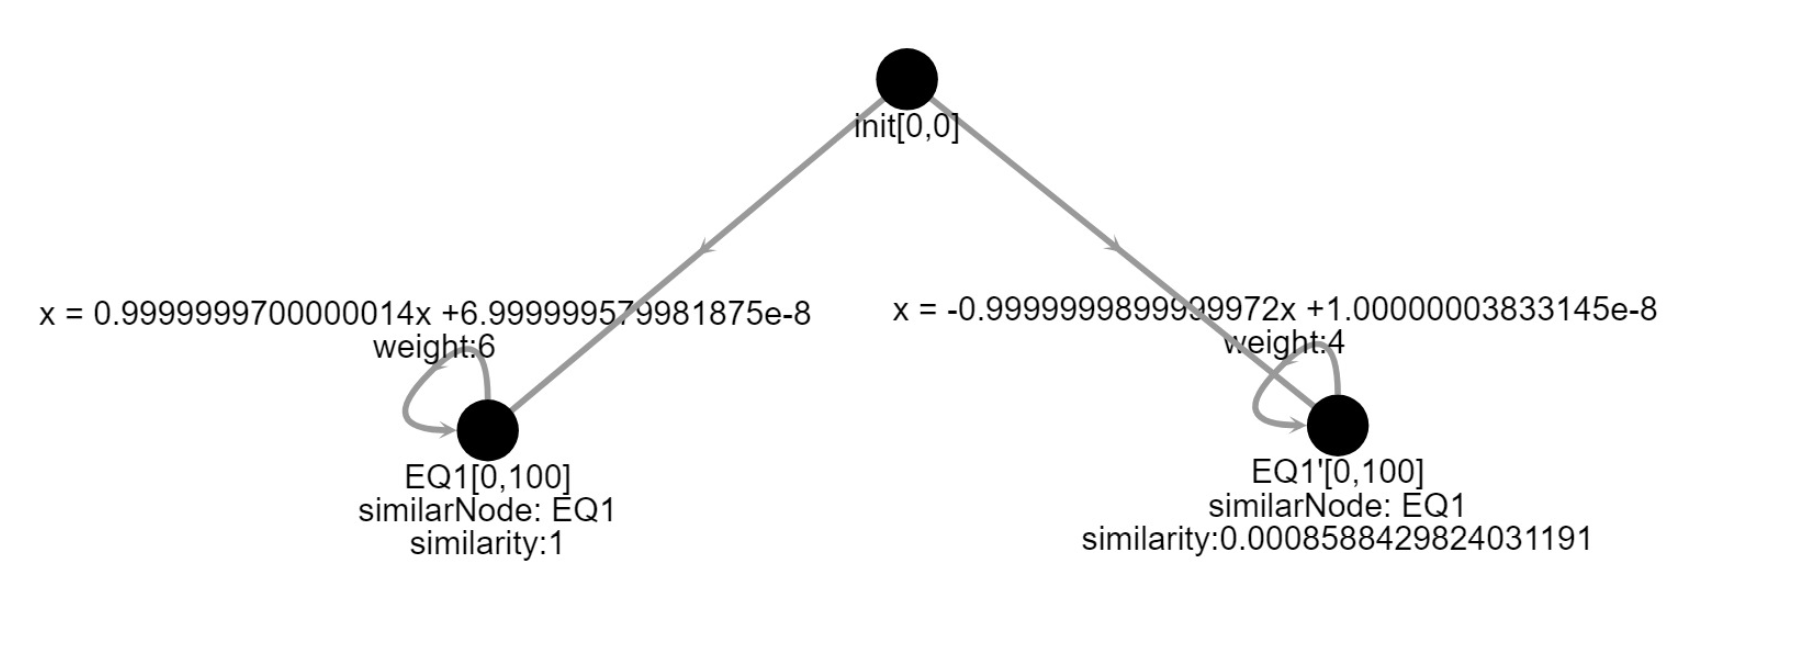
\includegraphics[scale=0.4]{./pictures/simple_experiment/learnedModel_branched_far.png}
	\caption{Sub-Experiment 2 - Branched Model}
	\label{combination_experiment_simple_1}
\end{figure}

\begin{figure}[h]
	\centering
	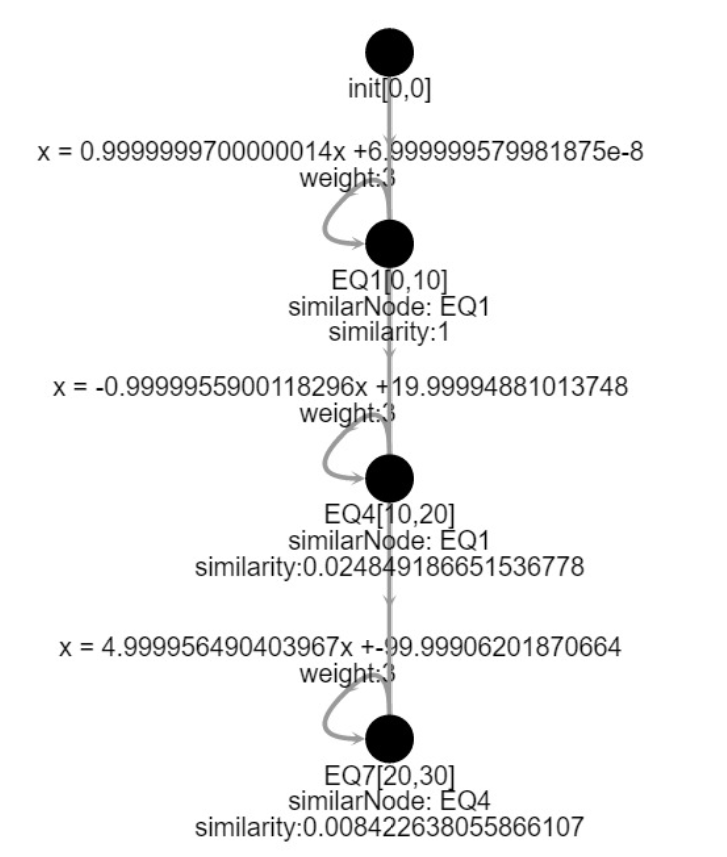
\includegraphics[scale=0.4]{./pictures/simple_experiment/learnedModel_sequential_far.png}
	\caption{Sub-Experiment 2 - Sequential Model}
	\label{combination_experiment_simple_2}
\end{figure}

\subsubsection{ Results}
We can see very positive results from both models in Table \ref{table:combination_simple_1} and Table \ref{table:combination_simple_2}, as it was always the case that the original models were sucessfully learned. This happens because the nodes from both models are relatively far and can be easily identified by the implementation with the calculation of their normalized Euclidean distances (e.g. similarity value). For example, one can see in Figure \ref{combination_experiment_simple_1} that the similarity value between \textit{EQ1} and \textit{EQ1'} is of approximately 0.00085. This value is always lower than the similarity threshold, as the last one can only be as low as 0.1. Meaning that the nodes from the previous models can never be merged, due to their difference in functionality. For this particular set of models, the only possibility to merge nodes would be to lower the similarity threshold from 0.1 to a value very close to 0. The only disadvantage of setting parameters like the \textit{similarity threshold} to 0, is that it may cause the learning process to loose significant precision of the observations. It may also confuse the learning process and indicate that very different nodes should be merged, when in reality they should be treated as different nodes.
\newpage
\begin{table}[htbp]
	\centering
	\resizebox{0.5\textwidth}{!}{\begin{minipage}{\textwidth}
			\begin{tabular}{||c c c c c||}
				\hline
				Similarity Threshold & Time Cost & Functionality Cost & Location Cost & Graph Similarity  \\ [0.5ex] 
				\hline\hline
				0.1 & 0.1 & 0.1 & 0.1 & 1 \\ 
				\hline
				0.5 & 0.1 & 0.1 & 0.1 & 1 \\ 
				\hline
				1 & 0.1 & 0.1 & 0.1 & 1 \\ 
				\hline
				0.1 & 0.5 & 0.1 & 0.1 & 1 \\ 
				\hline
				0.5 & 0.5 & 0.1 & 0.1 & 1 \\ 
				\hline
				1 & 0.5 & 0.1 & 0.1 & 1 \\ 
				\hline
				0.1 & 1 & 0.1 & 0.1 & 1 \\ 
				\hline
				0.5 & 1 & 0.1 & 0.1 & 1 \\ 
				\hline
				1 & 1 & 0.1 & 0.1 & 1 \\ 
				\hline
				0.1 & 0.1 & 0.5 & 0.1 & 1 \\ 
				\hline
				0.5 & 0.1 & 0.5 & 0.1 & 1 \\ 
				\hline
				1 & 0.1 & 0.5 & 0.1 & 1 \\ 
				\hline
				0.1 & 0.5 & 0.5 & 0.1 & 1 \\ 
				\hline
				0.5 & 0.5 & 0.5 & 0.1 & 1 \\ 
				\hline
				1 & 0.5 & 0.5 & 0.1 & 1 \\ 
				\hline
				0.1 & 1 & 0.5 & 0.1 & 1 \\ 
				\hline
				0.5 & 1 & 0.5 & 0.1 & 1 \\ 
				\hline
				1 & 1 & 0.5 & 0.1 & 1 \\ 
				\hline
				0.1 & 0.1 & 1 & 0.1 & 1 \\ 
				\hline
				0.5 & 0.1 & 1 & 0.1 & 1 \\ 
				\hline
				1 & 0.1 & 1 & 0.1 & 1 \\ 
				\hline
				0.1 & 0.5 & 1 & 0.1 & 1 \\ 
				\hline
				0.5 & 0.5 & 1 & 0.1 & 1 \\ 
				\hline
				1 & 0.5 & 1 & 0.1 & 1 \\ 
				\hline
				0.1 & 1 & 1 & 0.1 & 1 \\ 
				\hline
				0.5 & 1 & 1 & 0.1 & 1 \\ 
				\hline
				1 & 1 & 1 & 0.1 & 1 \\ 
				\hline
				0.1 & 0.1 & 0.1 & 0.5 & 1 \\ 
				\hline
				0.5 & 0.1 & 0.1 & 0.5 & 1 \\ 
				\hline
				1 & 0.1 & 0.1 & 0.5 & 1 \\ 
				\hline
				0.1 & 0.5 & 0.1 & 0.5 & 1 \\ 
				\hline
				0.5 & 0.5 & 0.1 & 0.5 & 1 \\ 
				\hline
				1 & 0.5 & 0.1 & 0.5 & 1 \\ 
				\hline
				0.1 & 1 & 0.1 & 0.5 & 1 \\ 
				\hline
				0.5 & 1 & 0.1 & 0.5 & 1 \\ 
				\hline
				1 & 1 & 0.1 & 0.5 & 1 \\ 
				\hline
				0.1 & 0.1 & 0.5 & 0.5 & 1 \\ 
				\hline
				0.5 & 0.1 & 0.5 & 0.5 & 1 \\ 
				\hline
				1 & 0.1 & 0.5 & 0.5 & 1 \\ 
				\hline
				0.1 & 0.5 & 0.5 & 0.5 & 1 \\ 
				\hline
				0.5 & 0.5 & 0.5 & 0.5 & 1 \\ 
				\hline
				1 & 0.5 & 0.5 & 0.5 & 1 \\ 
				\hline
				0.1 & 1 & 0.5 & 0.5 & 1 \\ 
				\hline
				0.5 & 1 & 0.5 & 0.5 & 1 \\ 
				\hline
				1 & 1 & 0.5 & 0.5 & 1 \\ 
				\hline
				0.1 & 0.1 & 1 & 0.5 & 1 \\ 
				\hline
				0.5 & 0.1 & 1 & 0.5 & 1 \\ 
				\hline
				1 & 0.1 & 1 & 0.5 & 1 \\ 
				\hline
				0.1 & 0.5 & 1 & 0.5 & 1 \\ 
				\hline
				0.5 & 0.5 & 1 & 0.5 & 1 \\ 
				\hline
				1 & 0.5 & 1 & 0.5 & 1 \\ 
				\hline
				0.1 & 1 & 1 & 0.5 & 1 \\ 
				\hline
				0.5 & 1 & 1 & 0.5 & 1 \\ 
				\hline
				1 & 1 & 1 & 0.5 & 1 \\ 
				\hline
				0.1 & 0.1 & 0.1 & 1 & 1 \\ 
				\hline
				0.5 & 0.1 & 0.1 & 1 & 1 \\ 
				\hline
				1 & 0.1 & 0.1 & 1 & 1 \\ 
				\hline
				0.1 & 0.5 & 0.1 & 1 & 1 \\ 
				\hline
				0.5 & 0.5 & 0.1 & 1 & 1 \\ 
				\hline
				1 & 0.5 & 0.1 & 1 & 1 \\ 
				\hline
				0.1 & 1 & 0.1 & 1 & 1 \\ 
				\hline
				0.5 & 1 & 0.1 & 1 & 1 \\ 
				\hline
				1 & 1 & 0.1 & 1 & 1 \\ 
				\hline
				0.1 & 0.1 & 0.5 & 1 & 1 \\ 
				\hline
				0.5 & 0.1 & 0.5 & 1 & 1 \\ 
				\hline
				1 & 0.1 & 0.5 & 1 & 1 \\ 
				\hline
				0.1 & 0.5 & 0.5 & 1 & 1 \\ 
				\hline
				0.5 & 0.5 & 0.5 & 1 & 1 \\ 
				\hline
				1 & 0.5 & 0.5 & 1 & 1 \\ 
				\hline
				0.1 & 1 & 0.5 & 1 & 1 \\ 
				\hline
				0.5 & 1 & 0.5 & 1 & 1 \\ 
				\hline
				1 & 1 & 0.5 & 1 & 1 \\ 
				\hline
				0.1 & 0.1 & 1 & 1 & 1 \\ 
				\hline
				0.5 & 0.1 & 1 & 1 & 1 \\ 
				\hline
				1 & 0.1 & 1 & 1 & 1 \\ 
				\hline
				0.1 & 0.5 & 1 & 1 & 1 \\ 
				\hline
				0.5 & 0.5 & 1 & 1 & 1 \\ 
				\hline
				1 & 0.5 & 1 & 1 & 1 \\ 
				\hline
				0.1 & 1 & 1 & 1 & 1 \\ 
				\hline
				0.5 & 1 & 1 & 1 & 1 \\ 
				\hline
				1 & 1 & 1 & 1 & 1 \\ [1ex] 
				\hline
				\hline
			\end{tabular}
	\end{minipage}}
	\caption{Sub-Experiment 2 - Branched Model Results}
	\label{table:combination_simple_1}
\end{table}

\begin{table}[htbp]
	\centering
	\resizebox{0.5\textwidth}{!}{\begin{minipage}{\textwidth}
			\begin{tabular}{||c c c c c||}
				\hline
				Similarity Threshold & Time Cost & Functionality Cost & Location Cost & Graph Similarity  \\ [0.5ex] 
				\hline\hline
				0.1 & 0.1 & 0.1 & 0.1 & 1 \\ 
				\hline
				0.5 & 0.1 & 0.1 & 0.1 & 1 \\ 
				\hline
				1 & 0.1 & 0.1 & 0.1 & 1 \\ 
				\hline
				0.1 & 0.5 & 0.1 & 0.1 & 1 \\ 
				\hline
				0.5 & 0.5 & 0.1 & 0.1 & 1 \\ 
				\hline
				1 & 0.5 & 0.1 & 0.1 & 1 \\ 
				\hline
				0.1 & 1 & 0.1 & 0.1 & 1 \\ 
				\hline
				0.5 & 1 & 0.1 & 0.1 & 1 \\ 
				\hline
				1 & 1 & 0.1 & 0.1 & 1 \\ 
				\hline
				0.1 & 0.1 & 0.5 & 0.1 & 1 \\ 
				\hline
				0.5 & 0.1 & 0.5 & 0.1 & 1 \\ 
				\hline
				1 & 0.1 & 0.5 & 0.1 & 1 \\ 
				\hline
				0.1 & 0.5 & 0.5 & 0.1 & 1 \\ 
				\hline
				0.5 & 0.5 & 0.5 & 0.1 & 1 \\ 
				\hline
				1 & 0.5 & 0.5 & 0.1 & 1 \\ 
				\hline
				0.1 & 1 & 0.5 & 0.1 & 1 \\ 
				\hline
				0.5 & 1 & 0.5 & 0.1 & 1 \\ 
				\hline
				1 & 1 & 0.5 & 0.1 & 1 \\ 
				\hline
				0.1 & 0.1 & 1 & 0.1 & 1 \\ 
				\hline
				0.5 & 0.1 & 1 & 0.1 & 1 \\ 
				\hline
				1 & 0.1 & 1 & 0.1 & 1 \\ 
				\hline
				0.1 & 0.5 & 1 & 0.1 & 1 \\ 
				\hline
				0.5 & 0.5 & 1 & 0.1 & 1 \\ 
				\hline
				1 & 0.5 & 1 & 0.1 & 1 \\ 
				\hline
				0.1 & 1 & 1 & 0.1 & 1 \\ 
				\hline
				0.5 & 1 & 1 & 0.1 & 1 \\ 
				\hline
				1 & 1 & 1 & 0.1 & 1 \\ 
				\hline
				0.1 & 0.1 & 0.1 & 0.5 & 1 \\ 
				\hline
				0.5 & 0.1 & 0.1 & 0.5 & 1 \\ 
				\hline
				1 & 0.1 & 0.1 & 0.5 & 1 \\ 
				\hline
				0.1 & 0.5 & 0.1 & 0.5 & 1 \\ 
				\hline
				0.5 & 0.5 & 0.1 & 0.5 & 1 \\ 
				\hline
				1 & 0.5 & 0.1 & 0.5 & 1 \\ 
				\hline
				0.1 & 1 & 0.1 & 0.5 & 1 \\ 
				\hline
				0.5 & 1 & 0.1 & 0.5 & 1 \\ 
				\hline
				1 & 1 & 0.1 & 0.5 & 1 \\ 
				\hline
				0.1 & 0.1 & 0.5 & 0.5 & 1 \\ 
				\hline
				0.5 & 0.1 & 0.5 & 0.5 & 1 \\ 
				\hline
				1 & 0.1 & 0.5 & 0.5 & 1 \\ 
				\hline
				0.1 & 0.5 & 0.5 & 0.5 & 1 \\ 
				\hline
				0.5 & 0.5 & 0.5 & 0.5 & 1 \\ 
				\hline
				1 & 0.5 & 0.5 & 0.5 & 1 \\ 
				\hline
				0.1 & 1 & 0.5 & 0.5 & 1 \\ 
				\hline
				0.5 & 1 & 0.5 & 0.5 & 1 \\ 
				\hline
				1 & 1 & 0.5 & 0.5 & 1 \\ 
				\hline
				0.1 & 0.1 & 1 & 0.5 & 1 \\ 
				\hline
				0.5 & 0.1 & 1 & 0.5 & 1 \\ 
				\hline
				1 & 0.1 & 1 & 0.5 & 1 \\ 
				\hline
				0.1 & 0.5 & 1 & 0.5 & 1 \\ 
				\hline
				0.5 & 0.5 & 1 & 0.5 & 1 \\ 
				\hline
				1 & 0.5 & 1 & 0.5 & 1 \\ 
				\hline
				0.1 & 1 & 1 & 0.5 & 1 \\ 
				\hline
				0.5 & 1 & 1 & 0.5 & 1 \\ 
				\hline
				1 & 1 & 1 & 0.5 & 1 \\ 
				\hline
				0.1 & 0.1 & 0.1 & 1 & 1 \\ 
				\hline
				0.5 & 0.1 & 0.1 & 1 & 1 \\ 
				\hline
				1 & 0.1 & 0.1 & 1 & 1 \\ 
				\hline
				0.1 & 0.5 & 0.1 & 1 & 1 \\ 
				\hline
				0.5 & 0.5 & 0.1 & 1 & 1 \\ 
				\hline
				1 & 0.5 & 0.1 & 1 & 1 \\ 
				\hline
				0.1 & 1 & 0.1 & 1 & 1 \\ 
				\hline
				0.5 & 1 & 0.1 & 1 & 1 \\ 
				\hline
				1 & 1 & 0.1 & 1 & 1 \\ 
				\hline
				0.1 & 0.1 & 0.5 & 1 & 1 \\ 
				\hline
				0.5 & 0.1 & 0.5 & 1 & 1 \\ 
				\hline
				1 & 0.1 & 0.5 & 1 & 1 \\ 
				\hline
				0.1 & 0.5 & 0.5 & 1 & 1 \\ 
				\hline
				0.5 & 0.5 & 0.5 & 1 & 1 \\ 
				\hline
				1 & 0.5 & 0.5 & 1 & 1 \\ 
				\hline
				0.1 & 1 & 0.5 & 1 & 1 \\ 
				\hline
				0.5 & 1 & 0.5 & 1 & 1 \\ 
				\hline
				1 & 1 & 0.5 & 1 & 1 \\ 
				\hline
				0.1 & 0.1 & 1 & 1 & 1 \\ 
				\hline
				0.5 & 0.1 & 1 & 1 & 1 \\ 
				\hline
				1 & 0.1 & 1 & 1 & 1 \\ 
				\hline
				0.1 & 0.5 & 1 & 1 & 1 \\ 
				\hline
				0.5 & 0.5 & 1 & 1 & 1 \\ 
				\hline
				1 & 0.5 & 1 & 1 & 1 \\ 
				\hline
				0.1 & 1 & 1 & 1 & 1 \\ 
				\hline
				0.5 & 1 & 1 & 1 & 1 \\ 
				\hline
				1 & 1 & 1 & 1 & 1 \\ [1ex] 
				\hline
				\hline
			\end{tabular}
	\end{minipage}}
	\caption{Sub-Experiment 2 - Sequential Model Results}
	\label{table:combination_simple_2}
\end{table}

